% Options for packages loaded elsewhere
% Options for packages loaded elsewhere
\PassOptionsToPackage{unicode}{hyperref}
\PassOptionsToPackage{hyphens}{url}
\PassOptionsToPackage{dvipsnames,svgnames,x11names}{xcolor}
%
\documentclass[
  11pt,
]{article}
\usepackage{xcolor}
\usepackage[margin=1in]{geometry}
\usepackage{amsmath,amssymb}
\setcounter{secnumdepth}{5}
\usepackage{iftex}
\ifPDFTeX
  \usepackage[T1]{fontenc}
  \usepackage[utf8]{inputenc}
  \usepackage{textcomp} % provide euro and other symbols
\else % if luatex or xetex
  \usepackage{unicode-math} % this also loads fontspec
  \defaultfontfeatures{Scale=MatchLowercase}
  \defaultfontfeatures[\rmfamily]{Ligatures=TeX,Scale=1}
\fi
\usepackage{lmodern}
\ifPDFTeX\else
  % xetex/luatex font selection
\fi
% Use upquote if available, for straight quotes in verbatim environments
\IfFileExists{upquote.sty}{\usepackage{upquote}}{}
\IfFileExists{microtype.sty}{% use microtype if available
  \usepackage[]{microtype}
  \UseMicrotypeSet[protrusion]{basicmath} % disable protrusion for tt fonts
}{}
\usepackage{setspace}
\makeatletter
\@ifundefined{KOMAClassName}{% if non-KOMA class
  \IfFileExists{parskip.sty}{%
    \usepackage{parskip}
  }{% else
    \setlength{\parindent}{0pt}
    \setlength{\parskip}{6pt plus 2pt minus 1pt}}
}{% if KOMA class
  \KOMAoptions{parskip=half}}
\makeatother
% Make \paragraph and \subparagraph free-standing
\makeatletter
\ifx\paragraph\undefined\else
  \let\oldparagraph\paragraph
  \renewcommand{\paragraph}{
    \@ifstar
      \xxxParagraphStar
      \xxxParagraphNoStar
  }
  \newcommand{\xxxParagraphStar}[1]{\oldparagraph*{#1}\mbox{}}
  \newcommand{\xxxParagraphNoStar}[1]{\oldparagraph{#1}\mbox{}}
\fi
\ifx\subparagraph\undefined\else
  \let\oldsubparagraph\subparagraph
  \renewcommand{\subparagraph}{
    \@ifstar
      \xxxSubParagraphStar
      \xxxSubParagraphNoStar
  }
  \newcommand{\xxxSubParagraphStar}[1]{\oldsubparagraph*{#1}\mbox{}}
  \newcommand{\xxxSubParagraphNoStar}[1]{\oldsubparagraph{#1}\mbox{}}
\fi
\makeatother


\usepackage{longtable,booktabs,array}
\usepackage{calc} % for calculating minipage widths
% Correct order of tables after \paragraph or \subparagraph
\usepackage{etoolbox}
\makeatletter
\patchcmd\longtable{\par}{\if@noskipsec\mbox{}\fi\par}{}{}
\makeatother
% Allow footnotes in longtable head/foot
\IfFileExists{footnotehyper.sty}{\usepackage{footnotehyper}}{\usepackage{footnote}}
\makesavenoteenv{longtable}
\usepackage{graphicx}
\makeatletter
\newsavebox\pandoc@box
\newcommand*\pandocbounded[1]{% scales image to fit in text height/width
  \sbox\pandoc@box{#1}%
  \Gscale@div\@tempa{\textheight}{\dimexpr\ht\pandoc@box+\dp\pandoc@box\relax}%
  \Gscale@div\@tempb{\linewidth}{\wd\pandoc@box}%
  \ifdim\@tempb\p@<\@tempa\p@\let\@tempa\@tempb\fi% select the smaller of both
  \ifdim\@tempa\p@<\p@\scalebox{\@tempa}{\usebox\pandoc@box}%
  \else\usebox{\pandoc@box}%
  \fi%
}
% Set default figure placement to htbp
\def\fps@figure{htbp}
\makeatother





\setlength{\emergencystretch}{3em} % prevent overfull lines

\providecommand{\tightlist}{%
  \setlength{\itemsep}{0pt}\setlength{\parskip}{0pt}}



 
\usepackage[]{biblatex}
\addbibresource{references.bib}


\usepackage{hyperref}
\hypersetup{
  colorlinks=true,
  linkcolor=blue,
  urlcolor=blue,
  breaklinks=true,
  pdfborder={0 0 0}
}
\makeatletter
\@ifpackageloaded{caption}{}{\usepackage{caption}}
\AtBeginDocument{%
\ifdefined\contentsname
  \renewcommand*\contentsname{Table of contents}
\else
  \newcommand\contentsname{Table of contents}
\fi
\ifdefined\listfigurename
  \renewcommand*\listfigurename{List of Figures}
\else
  \newcommand\listfigurename{List of Figures}
\fi
\ifdefined\listtablename
  \renewcommand*\listtablename{List of Tables}
\else
  \newcommand\listtablename{List of Tables}
\fi
\ifdefined\figurename
  \renewcommand*\figurename{Figure}
\else
  \newcommand\figurename{Figure}
\fi
\ifdefined\tablename
  \renewcommand*\tablename{Table}
\else
  \newcommand\tablename{Table}
\fi
}
\@ifpackageloaded{float}{}{\usepackage{float}}
\floatstyle{ruled}
\@ifundefined{c@chapter}{\newfloat{codelisting}{h}{lop}}{\newfloat{codelisting}{h}{lop}[chapter]}
\floatname{codelisting}{Listing}
\newcommand*\listoflistings{\listof{codelisting}{List of Listings}}
\makeatother
\makeatletter
\makeatother
\makeatletter
\@ifpackageloaded{caption}{}{\usepackage{caption}}
\@ifpackageloaded{subcaption}{}{\usepackage{subcaption}}
\makeatother
\usepackage{bookmark}
\IfFileExists{xurl.sty}{\usepackage{xurl}}{} % add URL line breaks if available
\urlstyle{same}
\hypersetup{
  pdftitle={William's Update},
  pdfauthor={William Clinton Co},
  colorlinks=true,
  linkcolor={blue},
  filecolor={Maroon},
  citecolor={blue},
  urlcolor={blue},
  pdfcreator={LaTeX via pandoc}}


\title{William's Update}
\usepackage{etoolbox}
\makeatletter
\providecommand{\subtitle}[1]{% add subtitle to \maketitle
  \apptocmd{\@title}{\par {\large #1 \par}}{}{}
}
\makeatother
\subtitle{COMM 498}
\author{William Clinton Co}
\date{August 3, 2025}
\begin{document}
\maketitle
\begin{abstract}
This document presents updated materials based on William and Ilan's
meeting on August 1, 2025 and provides updates and recommendations for
the upcoming course COMM 498.
\end{abstract}

\renewcommand*\contentsname{Table of contents}
{
\hypersetup{linkcolor=}
\setcounter{tocdepth}{3}
\tableofcontents
}

\setstretch{1}
\section{Housekeeping}\label{housekeeping}

\begin{itemize}
\tightlist
\item
  William will meet with the Sauder Canvas assistant on Tuesday, August
  5, 2025, to finalize course setup.
\item
  He has updated the syllabus with key dates and incorporated feedback
  from Ilan.
\item
  He removed the case studies that Ilan indicated were not of interest.
\item
  A copy of the updated syllabus is available
  \href{https://github.com/WilliamClintC/Comm_498/blob/main/Slides/William_Update_Syllabus.docx}{here}.
\end{itemize}

\section{Slides}\label{slides}

\subsection{Class 1 Introduction}\label{class-1-introduction}

Possible additional reading on inequality and economic growth:
\href{https://cepr.org/voxeu/columns/impact-wealth-inequality-economic-growth-evidence-italy-during-its-structural}{The
Impact of Wealth Inequality on Economic Growth}.

\subsection{Class 2/3 Globalization and
Slowbalization}\label{class-23-globalization-and-slowbalization}

Possible additional reading on slowbalization and political
polarization:
\href{https://cepr.org/voxeu/columns/globalisation-backlash}{Globalisation
Backlash}.

\subsection{Class 4/5 Threats to globaalization and Gains and costs
fromm
trade}\label{class-45-threats-to-globaalization-and-gains-and-costs-fromm-trade}

Additional reading on Trump's 30-Day Tariff Sprint:
\href{https://www.pbs.org/newshour/show/economist-analyzes-trumps-trade-deals-as-tariff-deadline-approaches}{Economist
analyzes Trump's trade deals as tariff deadline approaches}.

Additional reading on Liberation Day tariffs:
\href{https://www.csis.org/analysis/liberation-day-tariffs-explained\#:~:text=In\%20a\%20Rose\%20Garden\%20event,place\%20a\%20universal\%2010\%20percent}{Liberation
Day Tariffs Explained}.

\subsection{Class 6 Trade
institutions}\label{class-6-trade-institutions}

Additional reading on transshipment and tariff-circumvention strategies:
\href{https://time.com/7300087/trump-us-vietnam-trade-deal-china-transshipments/}{Trump
US--Vietnam trade deal and China transshipments}.

\subsection{Class 8/9 Internatiliazation and
location}\label{class-89-internatiliazation-and-location}

\begin{itemize}
\tightlist
\item
  The shown graphic below can be updated to a more modern aesthetic
\end{itemize}

\begin{figure}[H]

\centering{

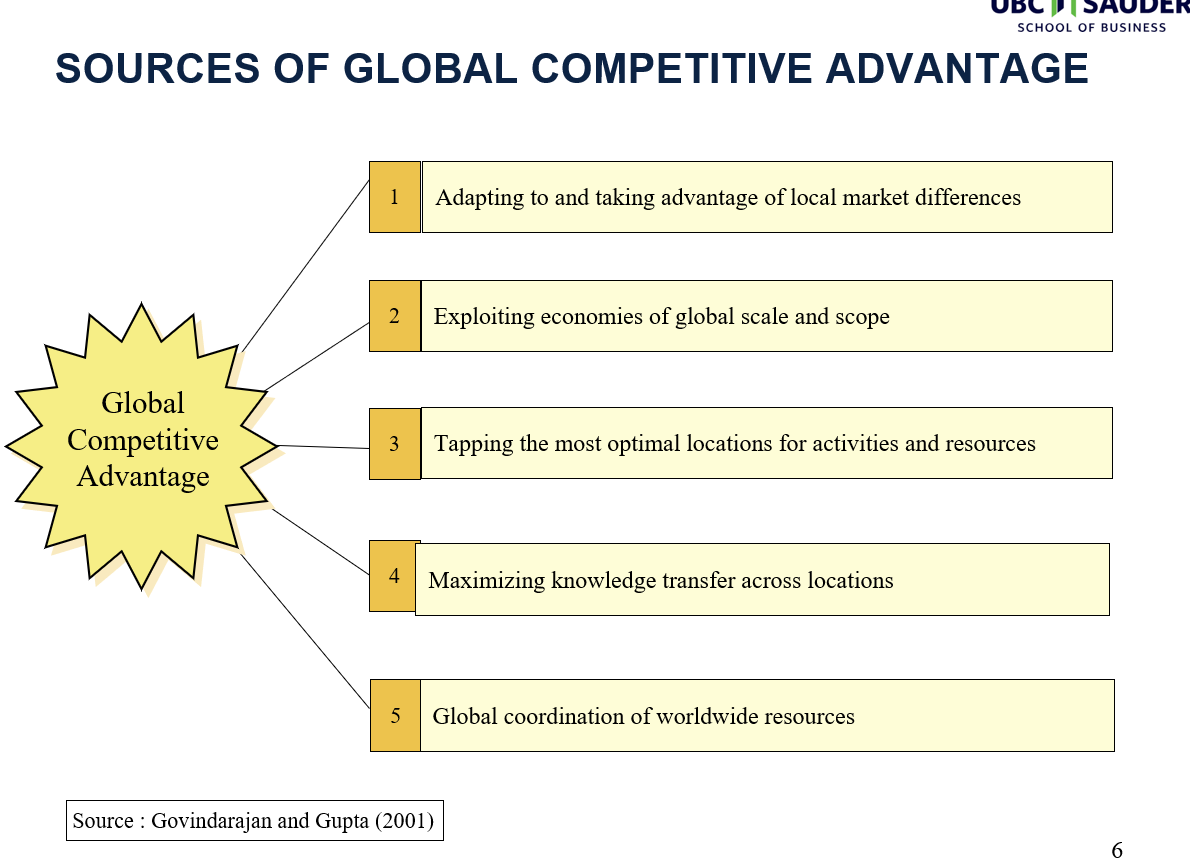
\includegraphics[width=0.8\linewidth,height=\textheight,keepaspectratio]{images/Screenshot 2025-08-02 013310.png}

}

\caption{\label{fig-1}2001 Graphic}

\end{figure}%

\begin{itemize}
\tightlist
\item
  Star TV case study maybe to dated (1993)
\end{itemize}

\subsubsection{Understanding Eastern
Culture}\label{understanding-eastern-culture}

\paragraph{Ebay}\label{ebay}

\begin{itemize}
\tightlist
\item
  Possible more recent study:
  \href{https://www.forbes.com/sites/helenwang/2010/09/12/how-ebay-failed-in-china/}{How
  eBay failed in China}
\item
  More analysis on eBay's China failure:
  \href{https://psmag.com/economics/why-ebay-failed-in-china-taobao-swift-guanxi-60072/}{Why
  eBay failed in China -- Taobao, Swift Guanxi}
\end{itemize}

\paragraph{AirBNB}\label{airbnb}

\begin{itemize}
\tightlist
\item
  \href{https://uq.pressbooks.pub/airbnb-978-1-74272-321-1/chapter/airbnb-in-china-before-during-and-after-covid-19/}{Airbnb
  in China before, during, and after COVID-19}
\item
  \href{https://medium.com/eastora-insights/airbnbs-china-exit-strategic-missteps-in-a-complex-market-86a26602e08d}{Airbnb's
  China exit: Strategic missteps in a complex market}
\end{itemize}

\paragraph{Exercise}\label{exercise}

\begin{itemize}
\tightlist
\item
  Do a location grid exercise
\end{itemize}

\subsection{Class 13/14 FDI and M\&A}\label{class13-14}

\begin{itemize}
\tightlist
\item
  The shown graphic below can be updated to a more modern aesthetic
\end{itemize}

\begin{figure}[H]

\centering{

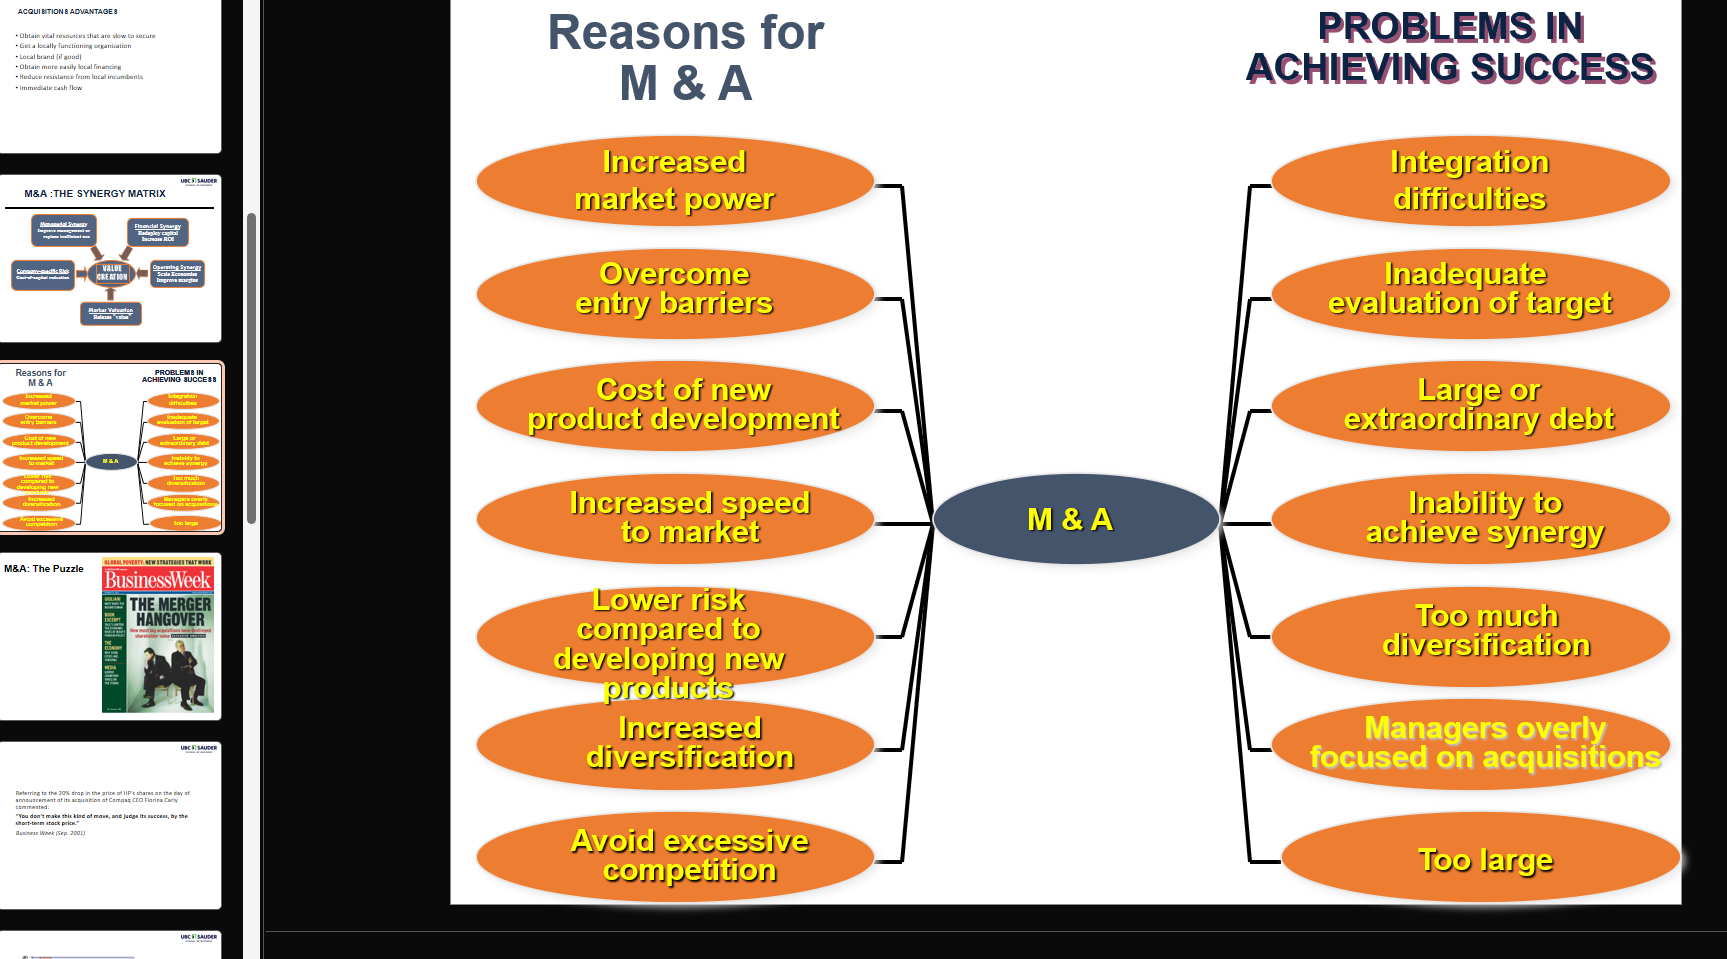
\includegraphics[width=0.8\linewidth,height=\textheight,keepaspectratio]{images/Screenshot 2025-08-02 021857.png}

}

\caption{\label{fig-2}Updated Modern Graphic}

\end{figure}%

\begin{itemize}
\tightlist
\item
  Discuss the Renault-Nissan joint venture:
  \href{https://knowledge.insead.edu/strategy/designing-durable-alliances-lessons-renault-nissan}{Designing
  Durable Alliances: Lessons from Renault-Nissan}.

  \begin{itemize}
  \tightlist
  \item
    \href{https://archive.ph/khRN8\#selection-1399.13-1419.71}{Another
    Source}
  \end{itemize}
\end{itemize}

\subsection{Class 11/12/16/17 Exporting, licsensing, global and regional
strategsion, tehcnological
disruptions}\label{class-11121617-exporting-licsensing-global-and-regional-strategsion-tehcnological-disruptions}

\begin{itemize}
\tightlist
\item
  This exercise is acceptable. No further improvements are needed; it is
  a reasonable exercise.
\end{itemize}

\subsection{Class 19 Political Risk}\label{class-19-political-risk}

Discuss the geopolitics of AI chips and related supply withholding
issues:

\begin{itemize}
\tightlist
\item
  \href{https://www.eetimes.com/ai-chip-controls-smuggling-and-geopolitics/}{AI
  Chip Controls, Smuggling, and Geopolitics}
\item
  \href{https://www.ft.com/content/a13ba438-3b43-46dd-b332-4b81b3644da0}{FT:
  AI Chip Export Controls}
\item
  \href{https://archive.ph/jcX8b\#selection-1999.6-2003.36}{Archived: AI
  Chip Geopolitics}
\end{itemize}

Discuss the politics of Didi's NYSE IPO and its aftermath:

\begin{itemize}
\tightlist
\item
  \href{https://www.europeanguanxi.com/post/didi-s-delisting-from-nyse-and-its-implications-explained}{Didi's
  Delisting from NYSE and Its Implications}
\item
  \href{https://www.atlanticcouncil.org/content-series/inflection-points/lessons-from-the-didi-ipo-ride-xi-faces-a-tradeoff-between-economic-dynamism-and-authoritarian-grip/}{Atlantic
  Council: Lessons from the Didi IPO}
\end{itemize}

Recent ICE Raids:

\begin{itemize}
\tightlist
\item
  \href{https://archive.ph/pp4xl}{Archived: ICE Raids}
\item
  \href{https://www.theguardian.com/us-news/2025/jul/29/trump-immigration-crackdown-labor-shortages-slowdowns}{Guardian:
  Trump Immigration Crackdown, Labor Shortages}
\end{itemize}

Tiktok Politics:

\begin{itemize}
\tightlist
\item
  \href{https://www.american.edu/sis/news/20250123-national-security-and-the-tik-tok-ban.cfm}{National
  Security and the TikTok Ban}
\item
  \href{https://apnews.com/article/tiktok-ban-biden-timeline-india-119969bfc584e92d47baa189a3e1c4fc}{AP
  News: TikTok Ban Timeline}
\end{itemize}

\subsection{Class 21/22/23 Cross Cultural
Management}\label{class-212223-cross-cultural-management}

\begin{itemize}
\tightlist
\item
  Revisit the Renault--Nissan joint venture case
  (\hyperref[class13-14]{Class 13/14}).
\item
  Discuss the role of religion in cross-cultural management practices.
\item
  Offtopic but it is a interesting story about the Colonel and Japan
  baseball:
  \href{https://www.cracked.com/article_44709_the-japanese-baseball-team-cursed-by-colonel-sanders.html}{The
  Curse of the Colonel (Cracked)} and
  \href{https://history.howstuffworks.com/american-history/ridiculous-history-curse-colonel.htm}{HowStuffWorks:
  The Ridiculous History of the Curse of Colonel Sanders}
\item
  \href{https://archive.ph/rR3Gt\#selection-565.3-593.46}{OpenAI in firm
  cultural clash}
\end{itemize}

\subsection{Class 24 Ethics}\label{class-24-ethics}

\subsubsection{Ethics of AI Use}\label{ethics-of-ai-use}

\begin{itemize}
\tightlist
\item
  IP and AI
  \href{https://theweek.com/tech/ai-fair-use-copyrighted-media-trains-bots}{The
  Week article on AI fair use}
\item
  Raytheon Ethics:
  \href{https://www.wsj.com/articles/rtx-agrees-to-more-than-280-million-in-penalties-to-settle-qatar-bribery-arms-control-violations-7368bf98?gaa_at=eafs&gaa_n=ASWzDAiE1z_s4buplQHYLUrzC8wR7x8ZeyDpQfmuQ1jNPC2pP_Jlvzp55qq7&gaa_sig=iVMI5Rj_kpBXM3-jcEi7EpdJeDq0X_0rZKIZSXoRcXHd1lx16d508-WH2zXsQ0gzXTPNK5K8Jg6y84RgOOK_IQ\%3D\%3D&gaa_ts=688be7a3}{RTX
  agrees to more than \$280 million in penalties to settle Qatar bribery
  \& arms control violations}
\item
  Glencore Ethics:
  \href{https://www.wsj.com/articles/inside-the-bribery-scandal-thats-sweeping-through-the-oil-industry-1518543648?gaa_at=eafs&gaa_n=ASWzDAjonC0ZvhOArbiu8fQmhaoIAPVBIEzyrt6edgKhfrs68TM_sYuKhM5b&gaa_sig=QXWvAA2pGRTO0SMy3UziYWQM3VHC4AgG7DTH-45eimDi-Yb7zFq2Z069trhFEsfSzIxNZ985EXf6nfVzo_nRKg\%3D\%3D&gaa_ts=688be7a3}{Inside
  the bribery scandal that's sweeping through the oil industry}
\item
  OpenAI ethical disputes within companies:
  \href{https://archive.ph/rR3Gt\#selection-565.3-593.46}{OpenAI in firm
  cultural clash}
\item
  Glencore Ethics:
  \href{https://www.wsj.com/articles/inside-the-bribery-scandal-thats-sweeping-through-the-oil-industry-1518543648?gaa_at=eafs&gaa_n=ASWzDAjonC0ZvhOArbiu8fQmhaoIAPVBIEzyrt6edgKhfrs68TM_sYuKhM5b&gaa_sig=QXWvAA2pGRTO0SMy3UziYWQM3VHC4AgG7DTH-45eimDi-Yb7zFq2Z069trhFEsfSzIxNZ985EXf6nfVzo_nRKg\%3D\%3D&gaa_ts=688be7a3}{Inside
  the bribery scandal that's sweeping through the oil industry}
\item
  OpenAI ethical disputes within companies:
  \href{https://archive.ph/rR3Gt\#selection-565.3-593.46}{OpenAI in firm
  cultural clash}
\end{itemize}

\subsection{Appendix}\label{appendix}

\begin{itemize}
\tightlist
\item
  \href{https://www.youtube.com/watch?v=NJuogMaLva4}{Details about
  Lawrence Jones Case}
\item
  I will be meeting with Sauder Canvas assistant this coming tuesday to
  add myself to canvas.
\end{itemize}

\section{William and Camille's Exercise
Recomndataions}\label{william-and-camilles-exercise-recomndataions}

\subsection{Roleplay}\label{roleplay}

students have now learned about how firms act when engaging in IB; they
should apply and test this knowledge in roleplay situations; professor
evaluates how effective their choices are and whether this accurately
reflects real decisions.

\subsubsection{Interactive trade or market entry
game}\label{interactive-trade-or-market-entry-game}

Turn international market analysis into a competitive activity where
teams act as firms choosing where to expand. Each country option has
different risk-reward profiles (tariffs, cultural barriers, supply chain
complexity), and teams justify their choices. Makes theoretical
frameworks more tangible. Acts as a low-stakes preliminary activity for
final project - gets students acquainted with this, may assist them in
ideation or execution of this project.

\subsubsection{International crisis response
simulation}\label{international-crisis-response-simulation}

Present a scenario involving a sudden geopolitical, economic, or
health-related disruption. Students take on roles (e.g., regional
director, risk analyst, COO) and collaborate to draft a real-time global
adaptation strategy (encourages fast thinking and practical
problem-solving.

\subsubsection{Final Project - International Expansion
Case}\label{final-project---international-expansion-case}

Objective: Apply strategic analysis tools to identify and solve a
company's core business challenges within an international context,
resulting in a recommendation that addresses both firm-specific and
global market dynamics

\subsubsection{Notes \& suggestions:}\label{notes-suggestions}

\begin{itemize}
\tightlist
\item
  Rubric could include section on presentation of case report (eg.
  visuals, organization of information, logical flow of report).
\item
  Could include contingency analysis: missing a risk assessment and plan
  to mitigate potential challenges.
\item
  Important to consider how implementation would vary under conditions
  of different nations (political situation, tastes, social \& economic
  factors)
\item
  Could include contingency analysis: missing a risk assessment and plan
  to mitigate potential challenges.
\item
  Important to consider how implementation would vary under conditions
  of different nations (political situation, tastes, social \& economic
  factors)
\end{itemize}


\printbibliography



\end{document}
